\documentclass[10pt]{article}
\usepackage{fontspec}
\setmainfont{lmroman10-regular.otf}[BoldFont=lmroman10-bold.otf,ItalicFont=lmroman10-italic.otf,BoldItalicFont=lmroman10-bolditalic.otf]
\setmonofont{lmmono10-regular.otf}
\usepackage[a4paper,margin=16mm,top=14mm,bottom=16mm]{geometry}
\usepackage{multicol,graphicx,xcolor,array,fancyhdr}
\usepackage[hidelinks]{hyperref}
\setlength{\columnsep}{6mm}
\setlength{\parindent}{1em}
\setlength{\parskip}{2pt}
\newcommand{\unk}[1]{\textcolor{red}{\texttt{\scriptsize[U+#1]}}}
\pagestyle{fancy}\fancyhf{}\renewcommand{\headrulewidth}{0.4pt}
\fancyhead[C]{\small MAGNETISM. \quad 129}
\begin{document}
\begin{multicols}{2}\raggedcolumns
% block 2 Text bbox=[0.0166, 0.0578, 0.0596, 0.1266]
41 tempered sheet from a the magma film.

% block 3 Text bbox=[0.0713, 0.0563, 0.4629, 0.1578]
But any degree of temper that is given to feed makes a very important change in this respect. In the first place, it acquires magnentifin more flowly by induction than an equal and similar piece of common iron, and its maly acquired lets. These differences are only transmined by the deviations which it causes in the manner’s needle from the magnetic meridian, and by its attractive tions.

% block 4 Text bbox=[0.0723, 0.1602, 0.4639, 0.2016]
When the inducing magnet is removed, fome magnetti remains in the fixed bar, which retains the polory which, it will be the neighborhood of the matter.

% block 5 Text bbox=[0.0732, 0.2023, 0.4648, 0.3484]
Steel tempered to the degree fit for watch Springs acquires along magnetic which is exhibits imme disels on the removal of the magnet. But it diffipates very fat ; and, in a very few minutes, it is reduced to lois than one half of its strength while in control with the magnet, and not two thirds of what it was distety on removal from it. It continues to diffidate for former days, though the her be kept with care'; but the diffusion diminishes at, and in the near at, half over third of its greatest power forany length of time, unleef cardially keep or indjudicially treated.

% block 6 Text bbox=[0.0586, 0.3477, 0.4619, 0.4266]
Steel tempered into flowing cutting tools, fish a schlieb, punches, and drills for metal, acquires magnifin fill more flowly by induction, and acquires five of it while in contact with the magnet, but it certain it more firms by, and finally retains a greater proportion of who it had acquired.

% block 7 Text bbox=[0.0576, 0.4273, 0.4658, 0.4945]
Steel made as hard as possible, is much longer in acquiring all the magnifin which limple juxtaposition can give to it. It acquires less than the formerly but it retains is with great firmness, and finally retains a much greater proportion.

% block 8 Text bbox=[0.0566, 0.4953, 0.4531, 0.8273]
Such one of iron as are fulcypible of magnetifi, are nearly like hard feel in their effects you that in the time necessary for their \_properlift\_ impregnation, and in the durability of the acquired magnifine. They effic exceedingly in respect to the degree of power which they can attain by mere juxtaption, and the virieties form to depend on heterogeneous mixture. We emit offriever, thus far once of our ones of influence of of magnetism of the metal in the fate of my way, and combred with dolphins, are not magnentable while remaining in that there. Mott core require reading, and a fort of cementation, in contact with inflammable fuhlances. This matter is not underdefended, but it would form that complex metallization is far from being the north to votrale condition, and that a certain degree of oxydation, and perhaps some other positive yet unknown, make the her lautiness. Our all this is extremely oblicure. The late Dr Cowin Knight made a compoliotion which required every phono and permanent magseting, but the recent died with him. Dr Gilbert peaks of limilat compositions, in which ferruginous days were ingredients ; but we know nothing of the fate of the metal in them, nor their mode of acquiring magretin.

% block 9 Text bbox=[0.0557, 0.8234, 0.4541, 0.9219]
It is of peculiar importance to work that the acquition of magnetization is gradual and progrestive, and that the gradation is the more perceptible in proportion as the field is of a hastheric temper. When a magnet is hrough to one end of a bar of common iron, to remote extremity, unleef exceedingly long, requires its utmost magnifin immediately. But when the north pole of

% block 10 Text bbox=[0.4668, 0.0508, 0.8682, 0.2547]
a magnet is applied: to one end of a bar of hard flee, the part in contact immediately becomes a fourth pole, and the far end is not yet affected. We offer a north pole formed a fance difference from the concept, and becsent that a faint tooth pole. "Their gradually advance along the bar. The remote extremity become frit a faint fourth pole, and it is not differ very long while (If ceer) that it becomes a simple, vigorous, north pole. More frequently it remains a difficult and recycle north pole: may, if the her for very long, it often hoppus that have a sacrifice of north and forth poles, which never make their way to the far end of the bar. This phenomenon was first observed (we think) by Dr Brook Taylor, who \_they\_ now account of his obtivations to the \_Philophysical Transformation\_, no 344.

% block 11 Text bbox=[0.4678, 0.2586, 0.8701, 0.4031]
From the account we have given of their phenomenons to a stof indeed magnifine, it appears that the temporary because magnifin is always lo disfpided that the rim of their beces mutual attractions of the difficiliate poles exceeds the gentich im of the repollon between the limlar, poles, and that therefore the two magnets tend to each other. This is evidently equivalent to flying, that a piece of magnungtic iron is always attracted by a magnet. No exception has ever been observed to this fact, for Phys's dury of a Thamades, or loadlines, which repeals iron, is allowed by all to have been a false.

% block 12 Text bbox=[0.4688, 0.4039, 0.8604, 0.5234]
We think outfellow authorified to lay that this attraction of the headlines for iron, or this tendency of iron to the headline, is a secondary phenomenon, and is the \_conference\_ of the proper disposition of the induced magnetimin. The proofs already given of the compound matters of this phenomena, namely, that is arise from the excess of two attributions above two repetitions, need (we imagine) no addition. But the following condiractions place the matter beyond doubt.

% block 13 Text bbox=[0.4697, 0.5242, 0.8711, 0.6422]
I. The magnifinal of the two poles is evidently of an opposite nature; the one repelling what the other attrade). If the aircraft iron, therefore, the other should result it. But each path, by changing a magretifion opposite to its own, on the nearest end of the iron, and the fans with its own on the remote end, and its action diminishing with an increase of diflants, there mult always be an excess of attraction, and the iron mult be attached.

% block 14 Text bbox=[0.4707, 0.6414, 0.8564, 0.8023]
A Each of the magnets A and B, in either of the positions reprefened in fig. 12. would alone attract the piece of common iron. But when placed together, the fourth pole of 8 tends to render the upper end of C a north pole; while the north pole of B tends to take it a South pole. If there actions be nearly equal, the weight of C cannot be supposedly be the magnifin induced by any difference of action that may remain. While C is hanging D I alone, let. A be gradually enough tree, it gradually thorley the action of the north pole of B, to that C gradually lofos its magnifin and polarity, and its weight prends.

% block 15 Text bbox=[0.4717, 0.8016, 0.8545, 0.9227]
§. He all three cases where the induction of magnetifism is flow, the attraction is weak in proportion. This is particularly remarked by Dr Gilbers. If we take piece of common iron, and of fleet of different temps, but all of the fame fine and form, we shall find that the iron is much more thought attracted than any of the rel, and that the attraction for each of them a weaker proportion as they are harder. This liberty is to accurately observed, that when the piece is thoroughly

% block 16 Caption bbox=[0.0781, 0.9203, 0.2627, 0.932]
\begin{center}\small\itshape Surez, Vol. II. Part I.\end{center}
% block 17 Picture bbox=[0.8008, 0.9234, 0.999, 0.9367]
\begin{center}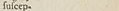
\includegraphics[width=\linewidth,height=0.45\textheight,keepaspectratio]{img/756-17.jpg}\end{center}
{\scriptsize\color{gray}\noindent Text inside picture (Parse): R\par}
\end{multicols}
\vfill\par\noindent\rule{\linewidth}{0.4pt}\par
{\scriptsize\color{gray}\noindent Source: Encyclopaedia Britannica scan, text from Parse 3.5 without correction. page\_id: britannica:309f765b1ecc83e0a7f7762e44b4a927a7555443:train:756 \quad row index: 756 \quad image sha256: 33eb91fcbe8d9d080f38ca26a23b791f56382bebff38a428cd4ac3cd30fb48f3 \quad parse model: nvidia/nemotron-3.5-parse \quad parse finish: stop \quad scan: \href{../scans/page-0756-33eb91fcbe8d.jpg}{page-0756-33eb91fcbe8d.jpg}\par}
\end{document}
